% --- CHAPTER 2: REQUIREMENTS ELICITATION AND ANALYSIS ---
\section{Requirements Elicitation and Analysis}
\label{sec:requirements}

This chapter establishes the formal operational boundaries of AdriaBOX, defining strictly \textit{what} the system must execute rather than \textit{how} its routines are programmatically concrete. Each requirement is mapped into a strict engineering specification to guarantee complete traceability during the software validation phase.

\subsection{Requirements Traceability Matrix}
To maintain a professional software engineering layout, the functional, non-functional, and implementation constraints are unified into a structural traceability ledger detailed in \Cref{tab:requirements_matrix}.

\begin{table}[htbp]
\small
\centering
\caption{AdriaBOX System Requirements Verification and Traceability Matrix}
\label{tab:requirements_matrix}
\vspace{2mm}
\begin{tabularx}{\textwidth}{l l p{3.2cm} X}
\toprule
\textbf{ID} & \textbf{Type} & \textbf{Target Component} & \textbf{Acceptance Criterion} \\
\midrule
\textbf{FR-1} & Functional & \texttt{server.py} / \texttt{core.py} & Unauthenticated resource endpoint requests must be rejected immediately with an HTTP 401 status code. \\
\textbf{FR-2} & Functional & \texttt{manager.py} & Uploading assets exceeding 64MB must slice the object into exactly $\lceil \text{Size}/64\text{MB} \rceil$ tracking metadata entries. \\
\textbf{FR-3} & Functional & \texttt{transfer.py} / \texttt{tcp.py} & Each logical block must stream through 3 unique nodes; connection drops mid-pipeline must abort the transaction. \\
\textbf{FR-4} & Functional & \texttt{db.py} / \texttt{manager.py} & Directory prefix creation (\texttt{mkdir}) or path movement (\texttt{mv}) must update SQL row entries within sub-second thresholds. \\
\textbf{FR-5} & Functional & \texttt{server.py} / \texttt{db.py} & Account removal must atomically drop relational state rows and dispatch physical erasure codes to worker daemons. \\
\textbf{NFR-1} & Non-Functional & \texttt{crypto.py} & Key derivation must run in local user space using 100,000 PBKDF2 iterations; raw keys must never hit the network. \\
\textbf{NFR-2} & Non-Functional & \texttt{server.py} / \texttt{tcp.py} & Write operations are only visible to the filesystem registry after all 3 replication pipeline mirrors confirm disk write state. \\
\textbf{NFR-3} & Non-Functional & \texttt{cli.py} / \texttt{ui.py} & Interface layout queries (\texttt{adria ls}) must abstract cluster paths, showing a single virtualized filesystem tree. \\
\textbf{IR-1} & Implementation & \texttt{pyproject.toml} & Runtime modules and dependency constraints must be handled exclusively within an isolated, deterministic Poetry environment. \\
\bottomrule
\end{tabularx}
\end{table}

The internal logical dependency layout and cross-layer requirement constraints are visualized in the tracking hierarchy graph in \Cref{fig:requirements_matrix}.

\begin{figure}[htbp]
    \centering
    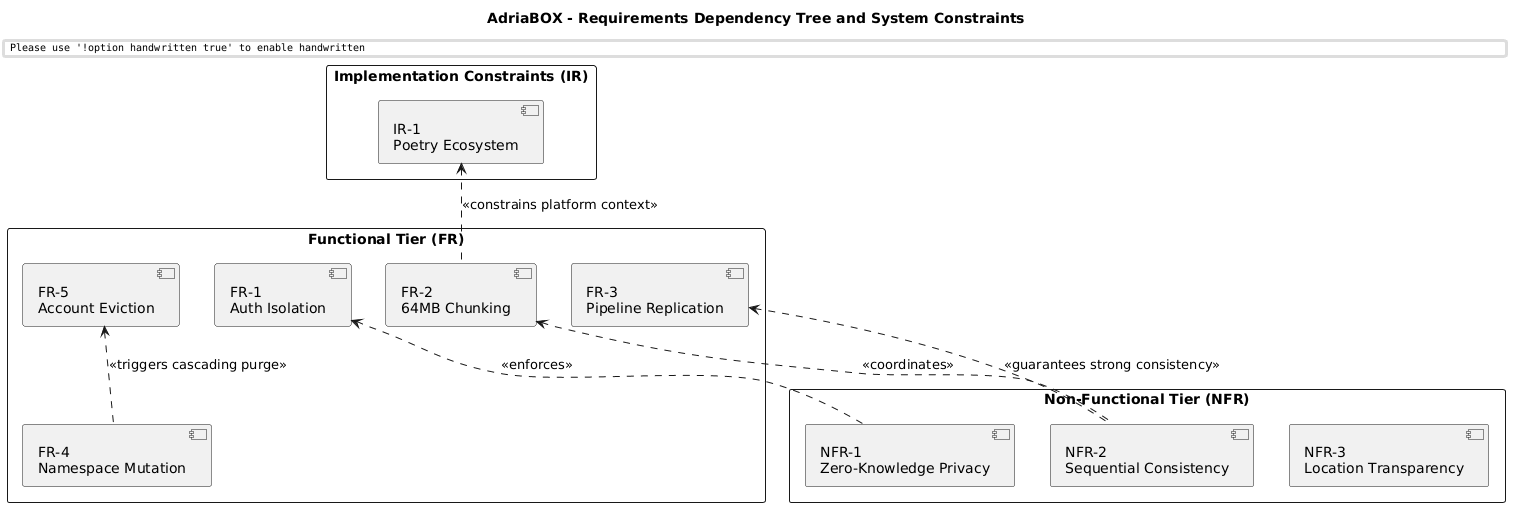
\includegraphics[width=0.85\textwidth]{plantuml/2.1-requirements-matrix.png}
    \caption{AdriaBOX System Requirements Dependency Layout and Operational Boundary Interconnection Map.}
    \label{fig:requirements_matrix}
\end{figure}

\subsection{Detailed Analysis of Functional Requirements}
The functional capabilities listed in the traceability matrix represent the operational baseline of the system. The authentication constraint (\textbf{FR-1}) isolates the metadata endpoints, forcing the application to validate credentials and evaluate signatures before authorizing access to the cluster status or user spaces. The storage partitioning strategy (\textbf{FR-2}) handles large files by automatically executing logical slicing whenever a transfer exceeds the 64MB threshold. This process works in tandem with the replication pipeline (\textbf{FR-3}), which routes data chunks sequentially across three unique storage nodes to ensure fault tolerance. Namespace operations (\textbf{FR-4}) implement virtual file management by modifying string keys directly in the database, ensuring instantaneous, non-blocking execution. Finally, the administrative cleanup routine (\textbf{FR-5}) enforces complete data destruction by executing cascading purges that erase relational metadata records while broadcasting physical erasure commands to wipe raw blocks from the storage disks.

\subsection{Detailed Analysis of Non-Functional and Technical Constraints}
Non-functional parameters govern the behavioral safety, data privacy, and isolation quality of the cluster. The zero-knowledge privacy requirement (\textbf{NFR-1}) shifts all cryptographic computations to local user space, utilizing PBKDF2 key derivation to ensure that raw passwords and decryption keys are never exposed to the network or the cloud infrastructure. Data plane consistency (\textbf{NFR-2}) guarantees sequential metadata integrity by delaying commit acknowledgments until all replica endpoints confirm a successful write operation. This structural abstraction is supported by the location transparency requirement (\textbf{NFR-3}), which hides low-level networking and chunk distributions behind a clean, virtualized filesystem layout. On the operational layer, the platform context is locked within an isolated Poetry environment (\textbf{IR-1}), neutralizing configuration drift across separate deployments. Within the evaluation framework, this technical constraint is rigorously verified by enclosing individual tenant execution routines inside distinct container runtimes, ensuring that state files, cached tokens, and memory-mapped cryptographic contexts are completely isolated within private user-space boundaries.

\subsection{Domain-Specific Technical Glossary}
\begin{itemize}
    \item \textbf{Object Key Prefix Alignment:} The method of embedding folder designations as text string tokens preceding an asset filename string within a flat database namespace registry.
    \item \textbf{Logical Partition Slicing:} The structural division of an un-fragmented binary asset stream into discrete data payloads matching an invariant architectural size boundary.
    \item \textbf{User-Space Staging Buffer:} A fixed allocation of process memory (RAM) used to hold raw data fragments moving between physical storage disks and network interface channels.
    \item \textbf{Zero-Knowledge Cryptography:} An infrastructure design protocol which guarantees that a data storage service provider does not possess the keys or plaintext blocks owned by its tenants.
    \item \textbf{Network Byte Order Formatting:} The Big-Endian integer arrangement requirement used to serialize multi-byte header fields across transport channels, ensuring compatibility across different processor setups.
\end{itemize}

\subsection{Architectural Analysis of the CAP Theorem and Distributed Features}
Engineering a decentralized data system requires an evaluation of the CAP Theorem (Consistency, Availability, Partition Tolerance). Under network partition events ($P$), a distributed platform must choose between absolute data consistency ($C$) and un-interrupted system availability ($A$). AdriaBOX is designed as a strictly \textbf{CP-focused infrastructure}, prioritizing absolute data correctness and sequential metadata validity over uncoordinated uptime. The system maintains this structural stance through two central mechanisms:

\subsubsection{Authoritative Quorum Constraints}
To eliminate the risk of split-brain conflicts—where a broken network path divides the cluster into competing segments running separate operations—the control plane relies on a single source of truth. If multiple orchestrators are introduced, the active master node must be validated by a strict absolute majority quorum ($Q$) of the cluster network size ($N$):
$$Q = \left\lfloor \frac{N}{2} \right\rfloor + 1$$
If a network partition isolates a cluster segment away from the central master, client nodes are prevented from bypassing the controller to write directly to storage daemons. This preserves the absolute consistency of the relational tracking maps.

\subsubsection{Synchronous Replication Cascade}
When uploading file blocks, data must travel through a multi-tiered pipeline:
$$\text{Data Plane Stream Path: } \text{Client CLI} \longrightarrow \text{Node}_{\text{Primary}} \longrightarrow \text{Node}_{\text{Replica 2}} \longrightarrow \text{Node}_{\text{Replica 3}}$$
An upload is not flagged as valid or committed to the database when the data hits the first storage container. The confirmation signal (\texttt{ACK\_OK}) must travel back up through the entire pipeline in reverse order. If a network failure breaks the pipeline midway, the transaction aborts instantly, preventing data corruption or partial writes.

\subsection{Evaluation of Distributed System Characteristics}
\subsubsection{Transparency}
AdriaBOX provides high location and replication transparency. Users interact with a clean virtual filesystem layout via the client interface, completely unaware of how objects are sliced, which nodes hold specific data blocks, or how many backup copies exist across the cluster.

\subsubsection{Fault Tolerance and Dependability}
Fault tolerance is maintained by mirroring every data chunk across three independent failure domains. If a storage container crashes or a disk controller drops offline during a download operation, the client's transport module automatically catches the socket exception and shifts its connection pointer to an active backup replica address, maintaining data availability with zero data loss. In our local multi-container testbed, this resilience layer is rigorously stressed by forcefully dropping target daemon containers, proving that client-side failover routing handles network anomalies transparently.

\subsubsection{Security, Multitenancy, and Trust Boundaries}
The system enforces strict tenant isolation. Standard user roles are restricted by data ownership parameters built into the SQL engine, preventing accounts from discovering or interacting with assets owned by other tenants. Administrative paths are protected by multi-layered verification walls. Although administrators possess elevated structural privileges to audit overall cluster health and evict user accounts, they cannot view or read file data contents due to the client-side encryption layers.

\subsubsection{Performance and Concurrency Efficiency}
Decoupling the control plane from active data paths ensures low-latency performance. The master node only handles lightweight orchestration messages, leaving the individual storage daemons to process high-throughput data streams inside separate, concurrent execution threads. Low-level memory efficiency is guaranteed by enforcing a constant 4096-byte transfer page configuration across all network interfaces.

\subsubsection{Features Explicitly Excluded from the Project Scope}
\begin{itemize}
    \item \textbf{Openness and Interoperability:} The platform relies on a custom, application-framed network protocol optimized for high-performance internal communication. Compatibility with external object APIs (such as AWS S3 or OpenStack Swift) was excluded to keep code lines clean and lightweight.
    \item \textbf{Evolvability and Rolling Upgrades:} The prototype focuses on providing a single-version deployment layout for academic evaluation. Long-term schema updates or backward-compatible protocol modifications were omitted from the core implementation design.
    \item \textbf{Economy and Cloud Operational Costs:} System optimization focuses on maximizing memory safety and fault isolation. Variable commercial hosting rates, automated container scaling budgets, and energy efficiency metrics are outside the project's tracking criteria.
\end{itemize}